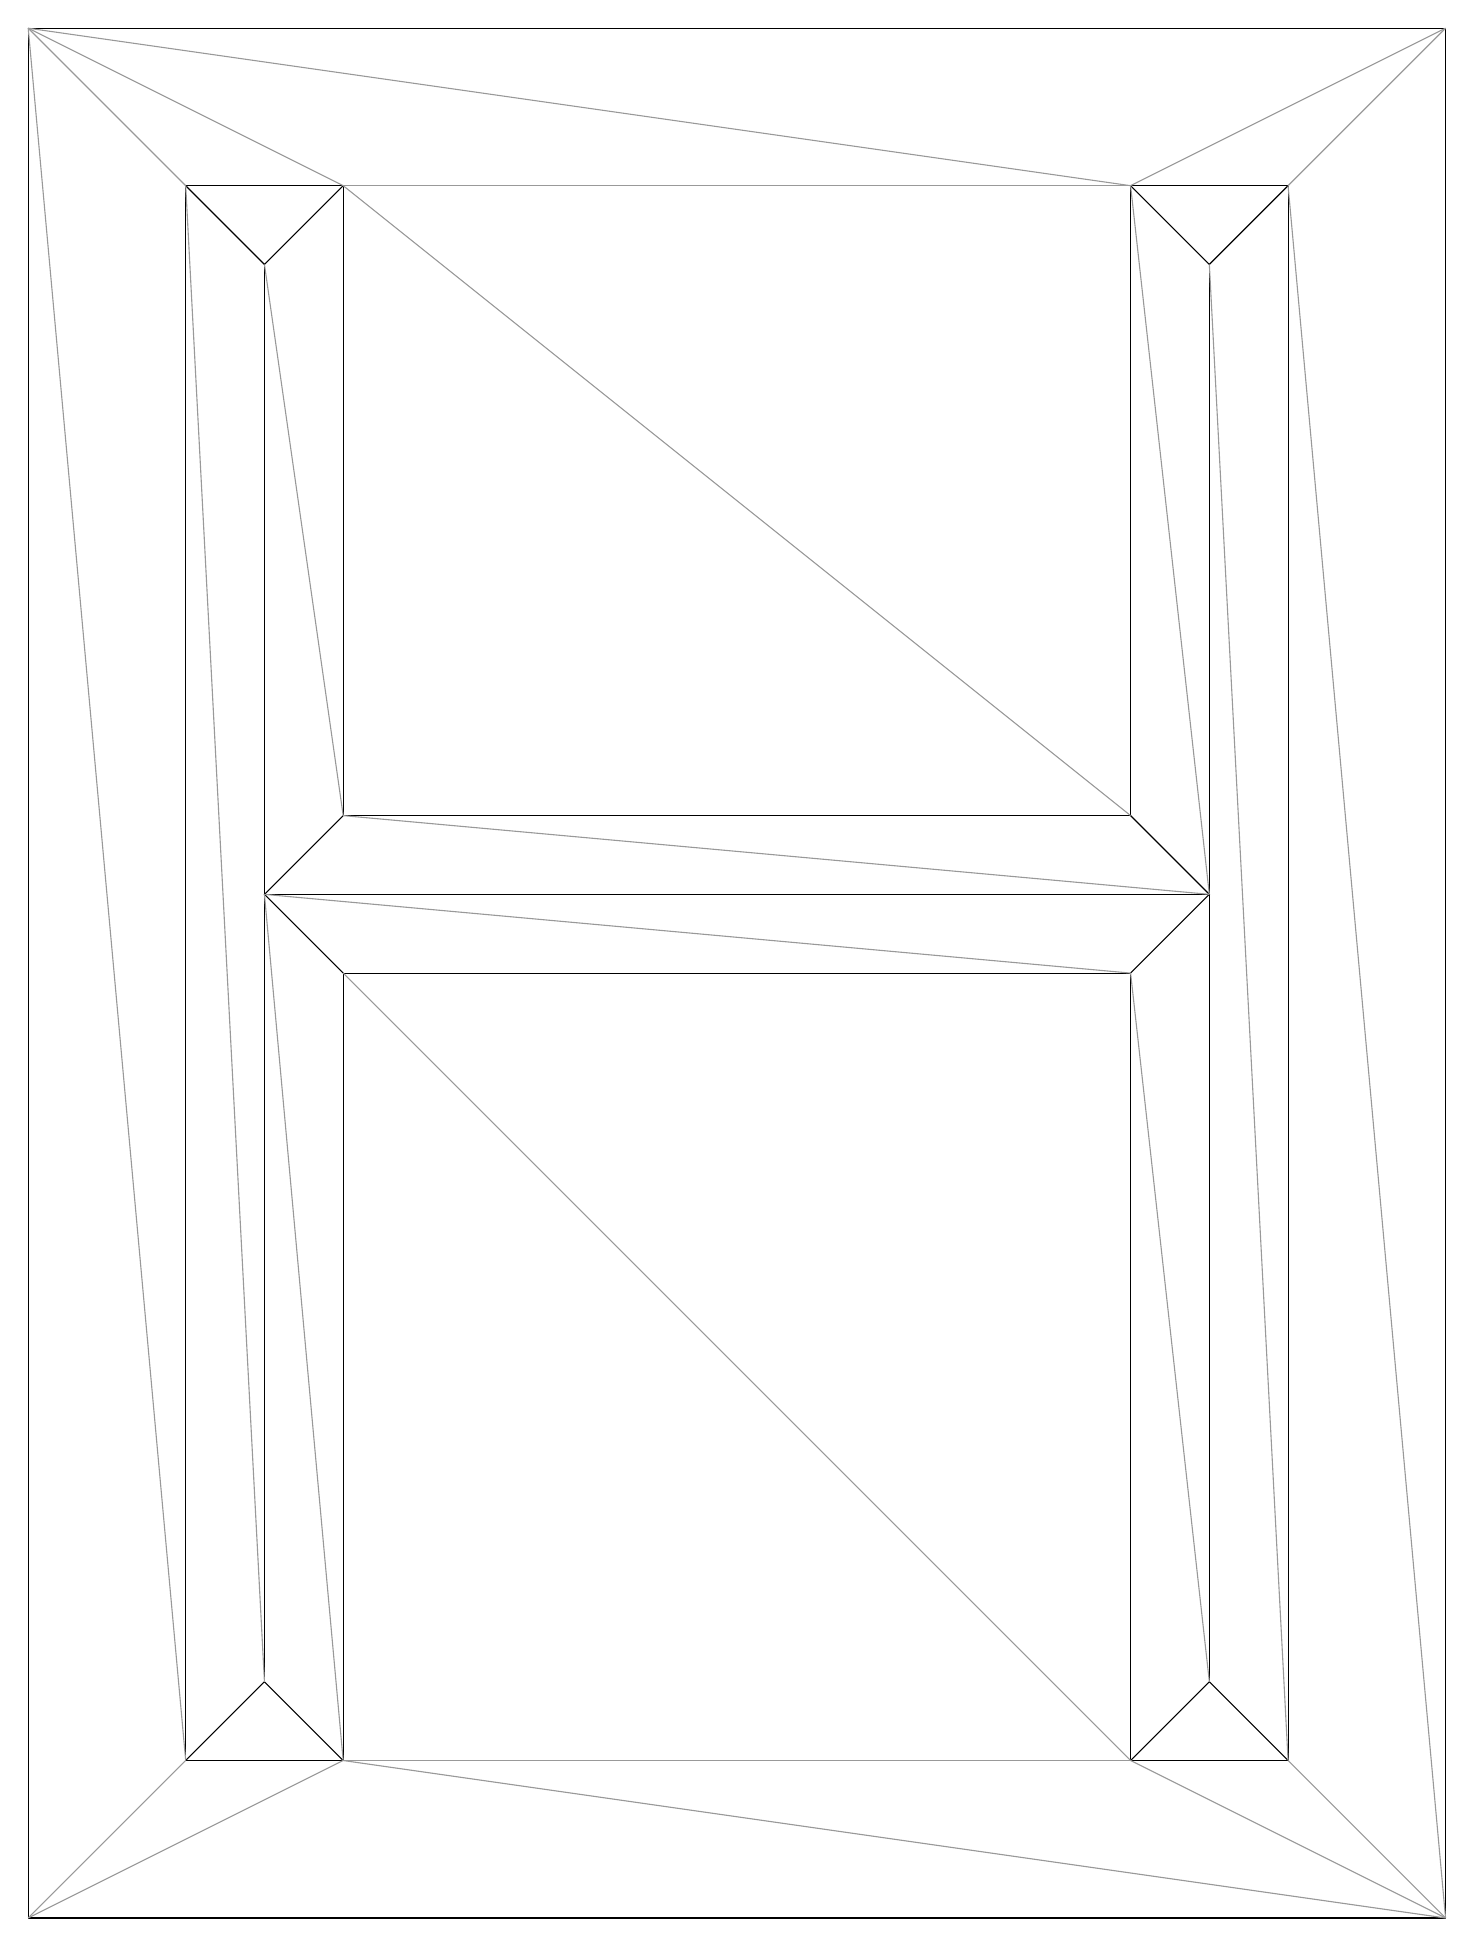
\begin{tikzpicture}
% Colors
\definecolor{outlineColor}{RGB}{0,0,0}
\definecolor{supportColor}{RGB}{153,153,153}
% Main H shape and Outline
\begin{scope}[outlineColor]
	\draw( 0, 0) % 0
	  -- ( 2, 0) % 1
	  -- ( 2,10) %12
	  -- (12,10) %13
	  -- (12, 0) % 2
	  -- (14, 0) % 3
	  -- (14,20) % 4
	  -- (12,20) % 5
	  -- (12,12) %14
	  -- ( 2,12) %15
	  -- ( 2,20) % 6
	  -- ( 0,20) % 7
	  -- cycle;  
	\draw( 0, 0) % 0
	  -- ( 1, 1) % 8
	  -- ( 2, 0);% 1
	\draw(12, 0) % 2
	  -- (13, 1) % 9
	  -- (14, 0);% 3
	\draw(14,20) % 4
	  -- (13,19) %10
	  -- (12,20);% 5
	\draw( 2,20) % 6
	  -- ( 1,19) %11
	  -- ( 0,20);% 7
	\draw( 2,10) %12
	  -- ( 1,11) %16
	  -- ( 2,12);%15
	\draw(12,10) %13
	  -- (13,11) %17
	  -- (12,12);%14
	\draw( 1, 1) % 8
	  -- ( 1,19);%11
	\draw(13, 1) % 9
	  -- (13,19);%10
	\draw( 1,11) %16
	  -- (13,11);%17
	\draw(-2,-2) %18
	  -- (16,-2) %19
	  -- (16,22) %20
	  -- (-2,22) %21
	  -- cycle;
\end{scope}
\begin{scope}[supportColor, thin]
	\draw( 0, 0) -- (-2,-2); % 0--18
	\draw( 0, 0) -- (-2,22); % 0--21
	\draw( 2, 0) -- (12, 0); % 1-- 2
	\draw( 2, 0) -- ( 1,11); % 1--16
	\draw( 2, 0) -- (-2,-2); % 1--18
	\draw( 2, 0) -- (16,-2); % 1--19
	\draw(12, 0) -- ( 2,10); % 2--12
	\draw(12, 0) -- (16,-2); % 2--19
	\draw(14, 0) -- (13,19); % 3--10
	\draw(14, 0) -- (16,-2); % 3--19
	\draw(14,20) -- (16,-2); % 4--19
	\draw(14,20) -- (16,22); % 4--20
	\draw(12,20) -- ( 2,20); % 5-- 6
	\draw(12,20) -- (13,11); % 5--17
	\draw(12,20) -- (16,22); % 5--20
	\draw(12,20) -- (-2,22); % 5--21
	\draw( 2,20) -- (12,12); % 6--14
	\draw( 2,20) -- (-2,22); % 6--21
	\draw( 0,20) -- ( 1, 1); % 7-- 8
	\draw( 0,20) -- (-2,22); % 7--21
	\draw(13, 1) -- (12,10); % 9--13
	\draw( 1,19) -- ( 2,12); %11--15
	\draw(12,10) -- ( 1,11); %13--16
	\draw( 2,12) -- (13,11); %15--17
\end{scope}
\end{tikzpicture}
